\documentclass[varwidth=9.7cm]{standalone}
\usepackage{pgfplots}
\pgfplotsset{compat=1.18}
\usepgfplotslibrary{statistics,groupplots}
\usepgflibrary{plotmarks, patterns}
\usetikzlibrary{calc, patterns, shapes}
\usepackage{xcolor}
\usepackage{pifont}
\newcommand{\cmark}{\ding{51}}  
\newcommand{\xmark}{\ding{55}}

\definecolor{ibm1}{HTML}{0077BB}
\definecolor{ibm2}{HTML}{33BBEE}
\definecolor{ibm3}{HTML}{EE7733}
\definecolor{ibm4}{HTML}{EE3377}
\definecolor{ibm5}{HTML}{CC3311}

\definecolor{grad1}{HTML}{364B9A}
\definecolor{grad2}{HTML}{98CAE1}
\definecolor{grad3}{HTML}{FEDA8B}
\definecolor{grad4}{HTML}{DD3D2D}
\definecolor{grad5}{HTML}{A50026}


\begin{document}

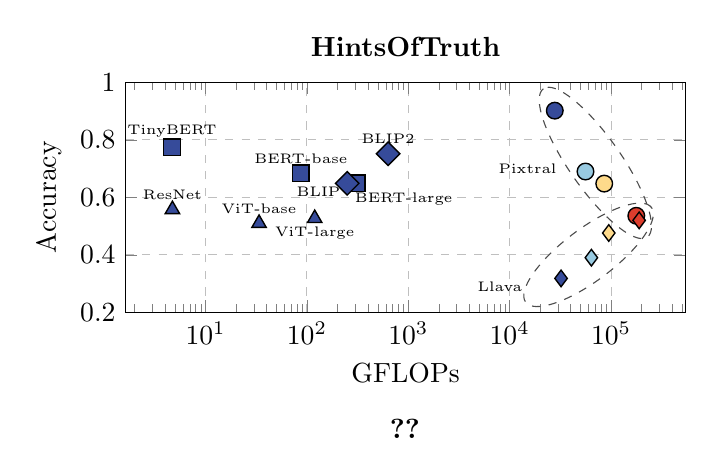
\begin{tikzpicture}

\begin{axis}[
    title={\textsc{\textbf{HintsOfTruth}}},
    name={budget-plot},
    xlabel={GFLOPs},
    width=8.7cm,
    height=4.5cm,
    ymajorgrids=true,
    xmajorgrids=true,
    grid style=dashed,
    legend to name=compute-legend,
    legend columns=4,
    legend style={
        draw=none,
    },
    ymin=0,
    xmode=log,
    ymax=1,
    ymin=0.2,
    ylabel={Accuracy},
    enlarge x limits=0.1,
    scatter/classes={
        0={mark=square*, rotate=45,   draw=black, fill=grad1},
        1={mark=square*,    draw=black, fill=grad1},
        2={mark=triangle*,  draw=black, fill=grad1},
        3={mark=diamond*,   draw=black, fill=grad1},
        4={mark=diamond*,   draw=black, fill=grad2},
        5={mark=diamond*,   draw=black, fill=grad3},
        6={mark=diamond*,   draw=black, fill=grad4},
        7={mark=*,  draw=black, fill=grad1},
        8={mark=*,  draw=black, fill=grad2},
        9={mark=*,  draw=black, fill=grad3},
        10={mark=*, draw=black, fill=grad4}
    }
]
\addlegendimage{area legend, 
               fill=grad1,
               draw=black,
               minimum width=3mm,
               minimum height=2mm}
\addlegendentry{0-shot}
\addlegendimage{area legend, 
               fill=grad2,
               draw=black,
               minimum width=3mm,
               minimum height=2mm}
\addlegendentry{1-shot}
\addlegendimage{area legend, 
               fill=grad3,
               draw=black,
               minimum width=3mm,
               minimum height=2mm}
\addlegendentry{2-shot}
\addlegendimage{area legend, 
               fill=grad4,
               draw=black,
               minimum width=3mm,
               minimum height=2mm}
\addlegendentry{5-shot}

\addplot[
    scatter, only marks,
    scatter src=explicit symbolic,
    mark size=3pt,
    mark options={line width=0.5pt},
] table[
    meta=model_type,                     % Reference label column
    x=x,
    y=y,
    header=true                          % Handle column headers
] {
    x    y    model_type    model_name
    4.67  0.775  1  TinyBERT
    87.02 0.684  1  BERT-base
    309.37 0.649 1  BERT-large
    4.71   0.558 2  ResNet
    33.71  0.510 2  ViT-base
    119.34 0.527 2  ViT-large
    249.58 0.649 0  BLIP
    631.59 0.752 0  BLIP2
    27843  0.902 7  Pixtral
    55943  0.690 8  Pixtral
    85630  0.648 9  Pixtral
    177391 0.536 10  Pixtral
    32117  0.318 3  Llava
    63963  0.390 4  Llava
    94930  0.476 5  Llava
    189197 0.520 6  Llava

};

\addplot+[
    scatter, only marks,
    scatter src=explicit symbolic,
    mark size=0pt,
    nodes near coords,                   % Auto-display metadata
    nodes near coords align={above},     % Position labels
    point meta=explicit symbolic,        % Enable text labels
    every node near coord/.style={
        anchor=south,
        font=\tiny,
        black
    },
] table[
    meta=model_name,                     % Reference label column
    col sep=space,                       % Specify space separator
    x=x,
    y=y,
    header=true                          % Handle column headers
] {
    x    y       model_name
    4.67   0.775 TinyBERT
    87.02  0.684 BERT-base
    309.37 0.649 {}
    4.71   0.558 ResNet
    33.71  0.510 ViT-base
    119.34 0.527 {}
    249.58 0.649 {}
    631.59 0.752 BLIP2
    
};

\node[] at (axis cs: 900, 0.595) {\tiny BERT-large};
\node[] at (axis cs: 130, 0.62) {\tiny BLIP};
\node[] at (axis cs: 119.34, 0.477) {\tiny ViT-large};
\node[ellipse,draw=black!70, dashed,minimum width=2cm, minimum height=.66cm,rotate=37] at (axis cs: 60000, 0.40) {};
\node[ellipse,draw=black!70, dashed,minimum width=2.3cm, minimum height=.66cm,rotate=125] at (axis cs: 70000, 0.72) {};
\node[] at (axis cs: 8000, 0.29) {\tiny Llava};
\node[] at (axis cs: 15000, 0.70) {\tiny Pixtral};

\end{axis}
\node[anchor=base] at (3.55cm,-1.6cm) {\ref{compute-legend}};


\end{tikzpicture}

\end{document}
